\begin{chapter}{Introdução}

\section{Contextualização}
Grande parte das tecnologias disponíveis no mercado já estão economicamente
acessíveis para uma grande parte da população. O uso de dispositivos eletrônicos
--- como os \textit{smatphones} e os computadores pessoais --- para o auxílio de
diversas tarefas tornou-se mais recorrente no cotidiano das pessoas. Com mais
pessoas utilizando essas ferramentas está surgindo inúmeras formas de melhorar a
interação entre usuários e aparelhos eletrônicos.

A comunicação entre pessoas e sistemas computacionais intensificou-se nas 
últimas décadas. Os desenvolvimentos tecnológicos alcançaram um estágio no qual
a interação humano-computador (IHC) incrivelmente está se assemelhando, por
exemplo, com a comunicação estabelecida entre duas pessoas. De fato, as máquinas
estão se aproximando do comportamento humano no sentido de serem capazes de
executarem tarefas semelhantes as ações de ouvir, entender, pensar e agir de
forma automática e independente. 

Apesar de todas as melhorias obtidas pela comunidade de pesquisa nos campos de
reconhecimento de padrões e \textit{design} de interface do usuário, as chamadas
interações convencionais~\cite{Preece15} ainda são as mais utilizadas para
controle de dispositivos. Por exemplo, \textit{mouse} e teclado são os
dispositivos de entrada mais utilizados em computadores de mesa, já que as telas
sensíveis ao toque são utilizados em \textit{smartphones} e \textit{tablets}. No
entanto, esses métodos de entradas convencionais forçam o usuário a utilizar as
mãos, o que se torna um problema sério se o usuário possuir algum problema na
realização de movimentos dos membros superiores --- que inclui também pessoas
com problemas em habilidades motoras finas, por exemplo, fraqueza dos dedos,
cujas limitações se concentram no manuseio de objetos físicos. Nesse sentido, as
interações não-convencionais devem ser exploradas a fim de evitar que pessoas
com deficiência motora sejam excluídas digitalmente. 

Interações não-convencionais, por definição, ocorrem quando o usuário é capaz de
se comunicar com um sistema computacional utilizando um dispositivo de
comunicação não tão comum, como câmeras, microfones, ou qualquer outro tipo de
sensor para entrada e/ou saída de dados~\cite{Machado10}. Por exemplo, pode-se
utilizar a fala como uma interação não-convencional para realizar uma tarefa de
digitação. Nesse caso, o dispositivo de entrada utilizado como método
convencional para realizar a digitação (normalmente um teclado) precisa ser
substituído por um microfone. Isso permite que tais equipamentos sejam
utilizados, portanto, como tecnologias assistivas, pois elas podem ser o único
caminho para que pessoas com deficiência motora dos membros superiores consigam
interagir autonomamente com dispositivos eletrônicos.

%Sistemas de reconhecimento ativo de gestos(AGR, do inglês \textit{actice gesture
%recognition})~\cite{Darrel96}, reconhecimento automático de voz (ASR, do inglês
%\textit{automatic speech recognition})~\cite{Taylor09}, síntese de voz (TTS, do inglês \textit{
%text-to-speech})~\cite{Huang01}, e acionadores externos são utilizados para melhorar a 
%interação humano-computador (IHC). Um sistema AGR é responsável por aplicar
%técnicas de computação visual para realizar o processamento \textit{frames} de
%vídeos de entrada e definir, então, na saída, qual a ação referente ao movimento
%motor realizado por uma determinada parte do corpo do usuário. O ASR é o sistema
%que recebe um sinal de fala digitalizado como entrada e gera um texto transcrito
%na saída. O sistema TTS possui a função de gerar um sinal de voz sintetizado a
%partir de um texto posto como entrada. Já os acionadores externos são
%equipamentos que auxiliam as pessoas com deficiência (PCD) a utilizarem
%aparelhos eletrônicos. Essas ferramentas ajudam  no controle de dispositivos
%eletrônicos promovendo comodidade e praticidade às pessoas e são normalmente
%enquadradas no conceito de Tecnologia Assistiva.

A Tecnologia Assistiva (TA) é uma área do conhecimento, de característica
interdisciplinar, que engloba produtos, recursos, metodologias, estratégias,
práticas e serviços que objetivam promover a funcionalidade, relacionada à
atividade e participação, de pessoas com deficiência, incapacidades ou
mobilidade reduzida, visando sua autonomia, independência, qualidade de vida e
inclusão social~\cite{cat09}.

Através da TA é possível reduzir as dificuldades vivenciadas por pessoas que
necessitam de soluções que não as deixem à margem da utilização de aparelhos
eletrônicos. Visando diminuir a exclusão digital imposta às pessoas com
deficiência (PCD) pela dificuldade ou total incapacidade para manipular certos
equipamentos, a acessibilidade é vista como elemento fundamental para elevar a
autoestima e o grau de independência dessas pessoas.

\section{Justificativa}

Segundo dados da Organização Mundial de Saúde (WHO, do inglês \textit{World
Health Organization}), aproximadamente 15\% da população mundial possui algum
tipo de deficiência~\cite{WHO15}. Esse número é realmente expressivo, pois
revela que, em uma população de 7,6 bilhões de pessoas, cerca de um sétimo
(1~bilhão de pessoas) é portadora de deficiência. A WHO também afirma que, em
2013, 80\% das pessoas com deficiência viviam em países ainda em
desenvolvimento, o que sugere que o predomínio da condição de deficiência está
bastante relacionado com a situação econômica dos países.

No Brasil, segundo o censo realizado em 2010 pelo Instituto Brasileiro de
Geografia e Estatística (IBGE), aproximadamente 23,9\% da população (cerca de
uma entre quatro pessoas, um total de 46~milhões de habitantes) declarou ter
alguma deficiência~\cite{tIBGE}. Os dados também mostram que, desse total, quase
7\% (cerca de de 13,2~milhões) apresentam dificuldades motoras. A
Tabela~\ref{tab:ibge} mostra o perfil da população brasileira com deficiência.

\begin{table}[!h]
\centering
\caption{Perfil da população brasileira com deficiência.}
\label{tab:ibge}
\def\arraystretch{1.25}
\begin{tabular}{lccr}
	\hline
	\hline
	\textbf{Deficiência} & \textbf{Descrição} & \textbf{Número de Pessoas} &
\textbf{Porcentagem} \\
	\hline
	Visual    & Cegueira ou dificuldades gerais   & 35.774.392  & 18,754 \%  \\
	Motora    & Paralisia ou dificuldades gerais  & 13.265.599  & 6,95 \% \\
	Auditiva  & Surdez ou dificuldades gerais     & 9.717.318   &  5,094 \%  \\
	Cognitiva & Problemas mentais ou intelectuais & 2.611.536   &  1,369 \%  \\ 
	\hline
	\hline
\end{tabular}
\end{table}

Apesar da atual existência de inúmeros instrumentos voltados para TA como
cadeiras de rodas e \textit{software} que facilitam a utilização de
computadores, grande parcela das PCD ainda não têm acesso a essas ferramentas. A
Organização Mundial de Saúde estima, por exemplo, que em países
subdesenvolvidos, aproximadamente 15\% das PCD têm acesso a essas Tecnologias
Assistivas\cite{WHO15}. Um fator que pode contribuir para esse cenário são os
altos preços de algumas dessas tecnologias. Os acionadores externos (dispositivos
de entrada que permitem as PCD a utilizarem equipamentos ativados normalmente por
botões ou teclados~\cite{tecla}), por exemplo, apesar de existir uma grande
variedade de tipos e funcionalidades, possuem um preço bem elevado. A
Tabela~\ref{tab:acionadores} mostra os preços de alguns acionadores externos
disponíveis no mercado. 
 
\begin{table}[!h]
\centering
\caption{Acionadores externos comerciais.}
\label{tab:acionadores}
\def\arraystretch{1.25}
\begin{tabular}{lcp{3cm}cp{3cm}}
	\hline
	\hline
	\textbf{Nome} & \textbf{Ref.} & \textbf{Método de acionamento} & \textbf{Comunicação} & \textbf{Custo (USD)} \\
	\hline
	Big Candy Corni        &~\cite{CandyCorn}        & Aproximação     & P2 Jack      & 215              \\
	Pal Pad                &~\cite{PalPad}           & Pressão         & P2 Jack      &  48 à 61         \\
	Jelly Bean             &~\cite{JellyBean}        & Pressão         & P2 Jack      &   65             \\
	Chin Switch            &~\cite{Chin}             & Pressão         & P2 Jack      & 220              \\
	Micro Light            &~\cite{MicroLight}       & Toque           & P2 Jack      & 85               \\ 
	HoneyBee               &~\cite{HoneyBee}         & Aproximação     & P2 Jack      & 149              \\
	AbleNet string Switch  &~\cite{StringSwitch}     & Puxa corda      & P2 Jack      & 65               \\
	Blue2 Switch           &~\cite{Blue2}            & Pressão         & Bluetooth    & 185              \\
	Savant Elite2          &~\cite{SavantElite2}     & Pressão         & USB          & 38 à 181         \\
	Foot Pedal             &~\cite{FootPedal}        & Pressão         & USB          & 267              \\
	Foot Switch            &~\cite{FootSwitch}       & Pressão         & USB          & 26               \\
	Sip/Puff Switch        &~\cite{SipPuff}          & Sopro ou sucção & USB          & 319              \\  
	
	\hline
	\hline
\end{tabular}
\end{table}

Acionadores que possuem como saída de comunicação o P2 Jack,
como~\cite{CandyCorn}, ~\cite{PalPad}, ~\cite{JellyBean}, ~\cite{Chin}, ~\cite{
MicroLight}, ~\cite{HoneyBee} e~\cite{StringSwitch}, são mais utilizados como
chaves para um determinado circuito. Um grande exemplo disso pode ser visto no
vídeo~\cite{ATswitchYT} que mostra a ativação da fala programada de uma boneca
através do pressionamento de um acionador. Como forma de controle de uma
determinada função do computador --- como o clique de um \textit{mouse} ---
através de um acionador externo, não foi encontrado nenhum dispositivo que
utiliza a comunicação P2 Jack conectado diretamente no computador que
realiza essa tarefa. É até possível controlar o clique de um mouse com a
comunicação P2 Jack, mas é necessário o auxílio de um \textit{mouse},
como~\cite{MouseJack}, mostrado na Figura~\ref{fig:mouse}, que possua uma
adaptação que receba como entrada o P2 Jack de um acionador. Já para
acionadores, como~\cite{Blue2}, ~\cite{SavantElite2}, ~\cite{FootPedal},
~\cite{FootSwitch} e ~\cite{SipPuff}, que possuem comunicação Bluetooth ou USB, 
conseguem realizar o controle dos evento de
clique de \textit{mouse} facilmente sem o auxílio de outros dispositivos,
bastando apenas realizar uma pequena configuração no próprio acionador.

\begin{figure}[!h]
	\centering
	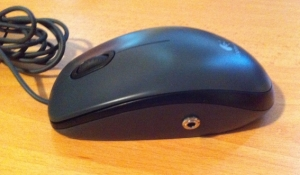
\includegraphics[width=0.5\textwidth]{fig/mouse13}
	\caption{Mouse adaptado para receber a interface P2 Jack de um acionador.}
	\label{fig:mouse}
\end{figure}

Como pode ser visto, o preço desses acionadores comerciais são bem elevados.
Alguns deles possuem um mecanismo bem simples e ainda assim são vendidos a preços
absurdos. Por exemplo, o acionador~\cite{StringSwitch}, como mostrado no
vídeo~\cite{videoStringSwitch}, possui apenas uma simples corda que puxa uma
chave de fim de curso. O pino de referência da chave é soldado no pino de
refêrencia do P2 Jack e o pino de estado da chave é soldado do pino se saída do
P2 Jack.  Assim, quando o corda do acionador é puxada, os pinos de referência e
saída do P2 Jack são curto circuitados, ``simulando'', no P2 Jack, os mesmos
estados de aberto e fechado da chave de fim de curso. Realizando pesquisas em
sites como MercadoLivre~\footnote{\url{https://www.mercadolivre.com.br/}}, é
possível encontrar a unidade de uma chave similar a utilizada nesse acionador
custando cerca de R\$ 2.50. Já o pino de P2 jack custa cerca de R\$ 1. Com esses
dois materiais é possível construir um acionador semelhante ao discutido
custando menos de R\$ 10, valor bem abaixo dos U\$ 65 cobrado por esse
acionador.

Na atual crise em que o Brasil se escontra, uma família de baixa renda, por
exemplo, difilcilmente iria adquidir um acionador externo devido ao elevedo
preço desses produtos, pois certamente comprometeria a renda mensal dessa
família.  Considernado que uma família possua a renda mensal de um salário
mínimo, e que esse salário está custando cerca de R\$ 954, e com o preço do
dólar custando R\$ 3.38, seria comprometido aproximadamente 23\% do salário
dessa família caso optassem por comprar esse acionador. Sendo assim, PCD de
baixa renda ficam impossibilitadas de adquirir esses produtos, excluindo-as de
usufruir de dispositivos que são voltadas para facilitar o uso de certos
equipamentos que não são adaptados para esse determinado público.

Nesse sentido, esta pesquisa tem como intuito apresentar uma solução para
diminuir a exclusão digital vivenciada pelas PCD, que muitas vezes não conseguem
utilizar aparelhos eletrônicos, como \textit{smartphones} e computadores, devido
a limitação de recursos que se adaptem às suas necessidades. Além disso a
solução proposta, apesar de ser voltada para o uso de uma determinada função em
aparelhos eletrônicos, como computador, pode ser utilizada em outros dispositivos
que necessitem de uma interação através do pressionamento de um botão, como
ligar ou desligar televisores. O uso de acionadores externos são bons
exemplos de dispositivos que auxiliam a utilização de diversos dispositivos,
porém como grande parte dos acionadores disponíveis no mercado possuem um custo
muito elevado, há a necessidade da solução proposta ser mais acessível
economicamente para que mais PCD possam ter acesso a essa ferramenta. % que
%auxiliam o uso de tarefas em dispositivos que normalmente não possuem interfaces
%alternativas de controle. 
 
\subsection{Trabalhos Relacionados}
A ideia de ajudar PCD a utilizar aparelhos eletrônicos com o auxílio de 
acionadores externos é alvo de inúmeras pesquisas. Uma grande parte dessas
pesquisas foca em auxiliar tarefas de controle das funções básicas do
\textit{mouse} de um computador. Para controlar o ponteiro do \textit{mouse},
geralmente utiliza-se os movimentos da cabeça ou dos olhos como método
não-convencional de controle. Para esse tipo de abordagem há uma certa
dificuldade em emular a função de clique.  Normalmente, para essa determinada
função,  é utilizada o \textit{dwelltime}, um método que utiliza um tempo
específico em segundos em que o ponteiro do mouse fica sobre um determinada área
da tela para realizar  o clique. Por exemplo, se o usuário posicionar o ponteiro
sobre o ícone de fechar uma aba de um navegador por um determinado tempo, irá
ser chamado a função de clique sobre esse ícone, fechando a aba do navegador. Um
dos problemas desse tipo de abordagem está no fato de que o usuário é obrigado a
ficar com a cabeça ou com os olhos parados em uma determinada posição por algum
tempo para que a função de clique seja ativada. Isso pode gerar um certo incômodo
no usuário, além de, naturalmente, aumentar o tempo de utilização a medida em
que o número de tarefas realizadas também aumentar.

Devido isso, há diversas pesquisas que tentam solucionar esse problema através de
métodos alternativos para a emulação do clique do \textit{mouse}.
Em~\cite{Aanand18} foi proposto um algoritmo chamado de OptiDwell para emular a
função de clique. Esse algoritmo utiliza o mesmo princípio do
\textit{dwelltime}, mas com a diferença de que o usuário sabe exatamente quando
o evento de clique irá acontecer. Utilizando o \textit{dwelltime} o usuário sabe qual é o
tempo específico em que o ponteiro deve ficar sobre uma área que se deseja
clicar, mas não tem a noção exata desse tempo. Por exemplo, se a pessoa deseja
pausar um vídeo no YouTube, ela deve posicionar o ponteiro sobre o ícone de
pause do vídeo e esperar o tempo de 2 segundos --- caso o \textit{dwelltime}
esteja configurado para 2 segundos --- para que a função de clique seja ativada.
Se em 1.99 segundos após ponteiro ficar sobre o ícone de pause, o cursor sair
dessa posição, a função de clique não é chamada, sendo necessário, então,
posicionar o ponteiro novamente em cima do ícone desejado. Com o algoritmo
OptiDwell, o usuário tem uma noção mais precisa do tempo para que a função de
clique seja realizada. O usuário sabe que o clique está para ser realizado
através da mudança de cor do cursor do \textit{mouse}. Por
exemplo, se a pessoa deseja clicar em uma letra no teclado virtual,
disponibilizado em vários sistemas operacionais, quando o ponteiro estiver sobre
uma determinada letra, a cor do ponteiro ficará mudando de cor ao longo do
tempo. Quando o ponteiro estiver em uma determinada cor, a função de clique será
chamada, além de ser ativado som de estalo (clique). Com isso a pessoa tem uma
noção mais precisa do tempo para realizar o clique, através de um
\textit{feedback} visual e sonoro. Contudo, o tempo de execução dessa função
continua sendo um problema, pois o tempo de execução de tarefas simples, como a
digitação, demanda bastante tempo e, com esse método, o tempo execução é bem maior
se comparado com outros métodos alternativos.

O trabalho proposto em~\cite{Skim10} utiliza um acionador baseado em dois
sensores ópticos: um LED (do inglês, ~\textit{light emitting diode})
infravermelho emissor e um receptor. Esse método levou em consideração o
clique simples e duplo, descartando a implementação da função ``clicar e
arrastar''. Os sensores foram posicionados bem próximos de um dos olhos do
usuário e através da tensão no LED infravermelho receptor foi possível
identificar se a pessoa estava de olho aberto ou fechado. Quando o usuário fica
de olho fechado há um certo sinal de tensão no LED receptor, mas quando o usuário
abre o olho, o sinal infravermelho refletido no olho aberto gera uma tensão, no
LED receptor, bem abaixo da tensão percebida quando a pessoa está com o olho
fechado. Com isso, foi possível detectar os eventos de clique identificando os
piscar dos olhos --- transição aberto-fechado dos olhos --- do usuário. A
detecção foi baseada na amplitude do sinal de tensão do LED receptor e o tempo
em que o usuário ficava de olho fechado, evitando que o sistema identificasse um
clique de involuntário quando a pessoa piscasse de forma natural. Esse acionador
construído para realizar o clique de um \textit{mouse} é bastante interessante,
porém, como descrito em~\cite{Batista17}, onde foi elaborado um acionador que
utiliza esse mesmo princípio de funcionamento, pode acarretar uma série de
reconhecimentos equivocados de clique devido o sensor utilizado ser bastante
influenciado pelas condições do ambiente, como iluminação de lâmpadas
fluorescentes e do sol.

O método proposto em~\cite{Karimullah02} utilizou o reconhecimento de voz para
controlar o ponteiro do \textit{mouse} e o evento de clique simples. Para a
movimentação do ponteiro, desenvolveu-se o reconhecimento para cinco comandos: \textit{move
left, move right, move up, move down} e \textit{stop}, para mover o cursor para
esquerda, direita, cima, baixo e parar o cursor, respectivamente. Quando o
usuário realiza um comando para mover o cursor, \textit{move right}, por 
exemplo, o ponteiro começa a se mover a 20 \textit{pixels} por segundo na
direção dado no comando e só para de se movimentar quando for reconhecido o
camando \textit{stop}. Em relação ao evento de clique, foi implementado apenas o
clique simples do \textit{mouse}, sendo necessário realizar o comando de voz 
\textit{click} para que o sistema emule essa função. O trabalho proposto é
bastante interessante, mas pode apresentar problemas, por exemplo, caso o usuário
desejar mover o cursor para uma determinada área que esteja muito próxima da
posição atual do ponteiro e não houver tempo suficiente entre os comandos de
mover e parar, o cursor pode não ficar exatamente sobre a área desejada.
Contudo, se a função de clique proposta pelo autor for combinada com outros
métodos alternativos de controle de \textit{mouse}, o tempo de realização das 
tarefas que envolvem o clique poderia ser mais otimizado.

Há trabalhos que utilizam acionadores baseados em sinais obtidos por
eletromiografia (EMG) --- um método de registro da atividade de um músculo quando
realiza contração~\cite{Amadio07} --- para implementar a função de clique.
Em~\cite{Pinheiro12}, por exemplo, foi implementado a função de clique simples e
duplo através de sinais de EMG. Os eletrodos que capturam os sinais elétricos
foram colocados no músculo frontal. A Figura~\ref{fig:frontal} mostra a
localização do músculo frontal. Para o clique simples, basta o usuário levantar
as sobrancelhas. Já para o clique duplo, a sobrancelha deve ser levantada duas
vezes de forma consecutiva. Assim, o sinal elétrico capturado pelo circuito de
EMG é convertido nesses dois eventos de clique.

\begin{figure}[!h]
	\centering
	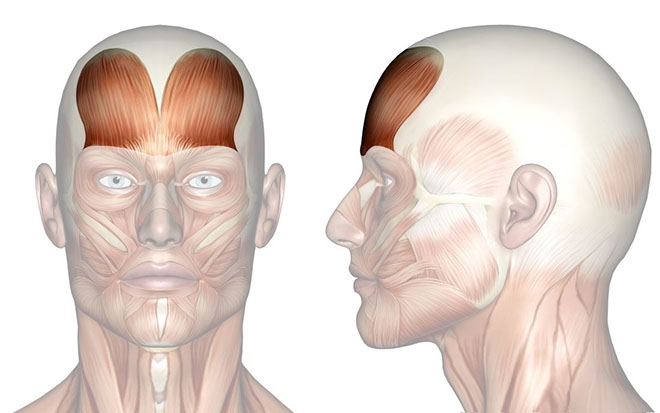
\includegraphics[width=0.5\textwidth]{fig/frontal}
	\caption{Músculo frontal.}
	\label{fig:frontal}
\end{figure}

Já em~\cite{Kaushik12} foi proposto um acionador que permitia controlar o
movimento do ponteiro do mouse e as funções de clique esquerdo e
direito, através de EMG e mecanomiografia (MMG). A MMG, é uma técnica
não-invasiva que registra as vibrações ou sons produzidos pelo músculo
esquelético ao se contrair~\cite{Vaz99}. Os eletrodos de EMG foram colocados nos
músculo masseter e risório, mostrados na Figura~\ref{fig:masseter} e na
Figura~\ref{fig:risorio}, respectivamente. %Para o MMG foi utilizado um
\begin{figure}[h!]
    \centering
    \begin{minipage}{.5\textwidth}
        \centering
        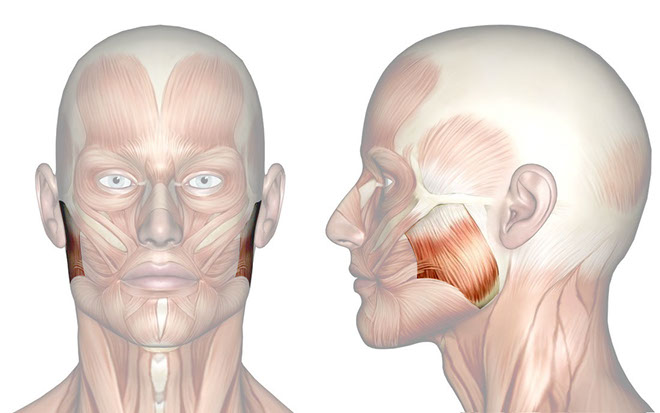
\includegraphics[width=0.91\linewidth, height=0.2\textheight]{fig/masseter}
        \caption{Músculo masseter.}
        \label{fig:masseter}
    \end{minipage}%
    \begin{minipage}{0.5\textwidth}
        \centering
        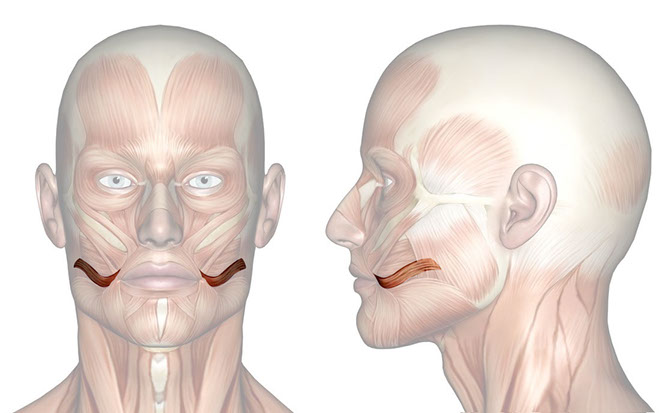
\includegraphics[width=0.91\linewidth, height=0.2\textheight]{fig/risorio}
        \caption{Músculo risório}
        \label{fig:risorio}
    \end{minipage}
\end{figure}
Para o MMG foi utilizado um Piezoelétrico --- um transdutor que sob estresses
mecânicos, como vibrações e compressões, gera sinais elétricos --- que foi
colocado no músculo platisma localizado no pescoço, como mostrado na
Figura~\ref{fig:platisma}. As palavras \textit{up, down, left} e \textit{right}
foram usadas para controlar o ponteiro do \textit{mouse}. Já para a função de
clique esquerdo e direito, foram utilizadas as palavras \textit{left click} e
\textit{right click}, respectivamente.
\begin{figure}[!h]
	\centering
	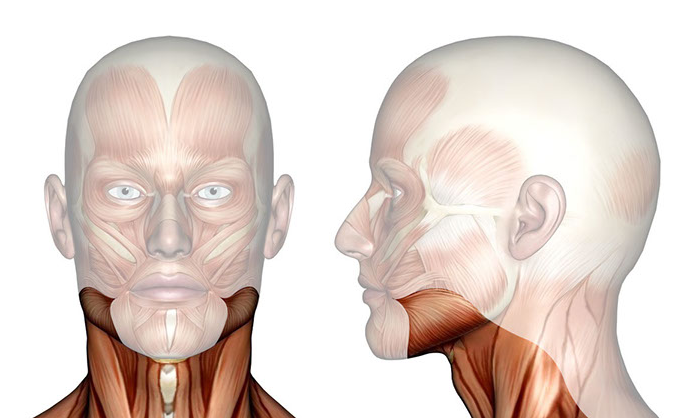
\includegraphics[width=0.5\textwidth]{fig/platisma}
	\caption{Músculo platisma.}
	\label{fig:platisma}
\end{figure}

O trabalho~\cite{Simpson08} realizou o controle do ponteiro através dos
movimentos da cabeça e utilizou um acionador muito interessante que
utilizava os sinais de um acelerômetro para realizar os eventos de clique. O
sensor acelerômetro foi posicionado atrás da orelha, de modo semelhante como
ficam posicionados alguns aparelhos auditivos que ajudam pessoas que possuem
dificuldade de audição a melhorar sua capacidade auditiva. Esse acionador é
dividido em dois módulos: transmissor e receptor. O módulo transmissor é o que
fica, de fato, posicionado atrás da orelha do usuário. Já o receptor fica
conectado diretamente no computador via USB. Os módulos se comunicam entre si
utilizando sinais de rádiofrequência. Para ativar a função de clique, o usuário
deve realizar uma pressão entre os dentes superiores e inferiores, de forma
semelhante como funciona a mastrigação. Portanto, quando o usuário realiza essa
pressão entre os dentes, é enviado um sinal do módulo transmissor, para o
receptor que, por sua vez, passa o comando referente ao clique para o computador
via USB. O sensor é capaz de distinguir o comando de clique através da pressão
entre os dentes, da vibração causada no sensor quando o usuário movimenta a
cabeça e até mesmo da vibração causada pelo ato de abrir a boca ao falar ou
bocejar. Isso evita que cliques sejam detectados de forma equivocada, tornando o
acionador mais confiável para o função do clique.

Já em~\cite{Antunes16} foi utilizado os movimentos da cabeça capturados por uma 
\textit{webcam} para controlar o ponteiro do mouse, sendo que, para o evento de
clique, foi utilizado o auxílio de um acionador baseado em pressão. O acionador
é do tipo pedal e é bem semelhante aos pedais utilizados por guitarristas para
realizar distorções em notas musicais produzidas pela guitarra. O acionador
possui uma comunicação direta com o computador através da tecnologia Bluetooth.
Para realizar um clique no computador, o usuário deve pressionar com
os pés o acionador. Quando o acionador é pressionado, o comando de clique é
enviado via Bluetooth para o computador.  Com isso, uma pessoa que tenha os
movimentos dos membros inferiores preservados, consegue utilizar a função de
clique no computador sem a necessidade de utilizar a mãos. 

Como visto até agora, existem diversos tipos de acionadores construídos com a
finalidade de serem utilizados como método alternativo para o clique do
\textit{mouse}.  Contudo, dentre a literatura consultada, não foi encontrado
nenhuma pesquisa na área acadêmica que utilizasse um acionador baseado em sopro
como interface para gerar comandos de clique para serem emulados no computador.
Até existem produtos no mercado com a proposta de controlar os eventos de
clique através do sopro, como o acionador Sip/Puff Switch~\cite{SipPuff} e o
IntegraMouse~\cite{IntegraMouse} --- um produto que permite controlar o ponteiro do
\textit{mouse} e realizar cliques no computador, através dos movimentos da boca
e de sopro, respectivamente. Entretanto, o Sip/Puff Switch custa cerca
de U\$ 319, já o IntegraMouse está custando em média \euro 2000. Esses preços
são extremamanete altos para pessoas de baixo poder aquisitivo. Esse alto preço
contribui bastante para que esse tipo de TA não seja
amplamente difundida, contribuindo para o aumento da exclusão digital imposta às
PCD.

Diante de tais circunstâncias, este trabalho tem como finalidade apresentar  uma
solução para diminuir a exclusão digital vivenciada por PCD, as quais estão à
margem do mundo eletrônico por conta da ausência de recursos que adaptem os
dispositivos às suas necessidades. Sendo assim, um acionador externo baseado em
sopro facilitaria o uso das funções de clique do \textit{mouse} para tarefas
executadas no computador e essa ferramenta seria utilizada em conjunto, por
exemplo, com um \textit{software} que capture imagens do rosto do usuário em
tempo real através de uma \textit{webcam} para controlar o movimento do cursor
do \textit{mouse} ao longo do monitor. Dessa forma, uma pessoa que antes não
conseguia utilizar um computador, poderá realizar várias tarefas no computador
de forma independente, ajudando na inclusão digital e social dessa pessoa.

\section{Objetivos}

O objetivo geral do projeto é construir um protótipo de acionador externo
baseado e sopro que ajude as PCD a controlarem de forma independente os eventos
de clique do \textit{mouse}. A principio, como prova de conceito, será possível
controlar os cliques apenas em sistemas operacionais Linux, como o Ubuntu e seus
derivados. No entanto, o sistema projetado pode ser ampliando para os sistemas
operacionais Windows e MacOS para atender um maior número de potenciais usuários
do produto. É importante também que esse produto seja de baixo custo e que todo
o projeto seja livremente disponibilizado, para que qualquer pessoa que tenha
acesso a esse projeto, se desejar, possa construir por conta própria seu
acionador, aumentando assim, o número de pessoas beneficiadas por este trabalho.

O protótipo deve ser colocado em uma posição próxima a boca do usuário com o auxílio
de um \textit{headset} modificado que servirá de suporte para ajudar o acionador
a ficar em uma posição ideal para que o usuário consiga realizar o sopro sem
dificuldades. A interface de comunicação do acionador com o computador será o
P2 Jack 3.5~mm para que a pessoa possa utilizar o mesmo acionador, que foi
projetado para usar a função de clique de um \textit{mouse}, em outro tipo de
contexto, como em brinquedos que precisam de um tipo de acionamento externo. Um
\textit{software} será desenvolvido para capturar os sinais da interface P2 Jack
e convertê-los em ações de clique no computador.

Testes com o protótipo serão aplicados a voluntários para verificar o potencial
do produto e verificar possíveis desvantagens para futuras melhorias.

\begin{subsection}{Objetivos Específicos}

Os objetivos específicos podem ser:
i) estudo e implementação das ferramentas que constituem acionador;
ii) estudo de APIs para criação do \textit{software};
iii) teste com voluntários;
iv) resultados.

Uma breve descrição sobre cada tópico é feita a seguir.

\begin{enumerate}[i)]

\setlength\itemsep{-.2cm}
	\item Estudo e implementação ferramentas que constituem o acionador: \vspace{-.2cm}
	\begin{itemize}
		%\setlength\itemsep{-.1cm}
		\item Estudo do efeito piezoelétrico;
		\item Estudo de circuito comparador com amplificadores operacionais;
		\item Construção circuito protótipo do acionador.
	\end{itemize}

	\item Estudo de APIs para a criação do \textit{software}: \vspace{-.2cm}
	\begin{itemize}
		%\setlength\itemsep{-.1cm}
		\item Estudo de APIs para captura de sinais da interface P2 Jack;
		\item Estudo de APIs que permitam manipular os eventos de clique;
		\item Implementação do \textit{software}.
	\end{itemize}

	\item Testes com voluntários: \vspace{-.2cm}
	\begin{itemize}
		%\setlength\itemsep{-.1cm}
		\item Cenário de testes compostos pelo método proposto e outro método alternativo para os eventos de clique;
		\item Aplicação de um questionário capaz de quantificar atributos qualitativos do sistema.
	\end{itemize}

	\item Resultados: \vspace{-.1cm}
	\begin{itemize}
		%\setlength\itemsep{-.1cm}
		\item Análise comparativa entre o método proposto e outro método alternativo de clique;
		\item vantagens e desvantagens do acionador;
		\item Indicação de trabalhos futuros.
	\end{itemize}

\end{enumerate}

\end{subsection}

\section{Síntese de Conteúdo}

Este capítulo fez uma breve introdução sobre as motivações que levaram ao
desenvolvimento do projeto além de mostrar os objetivos do trabalho.
A seguir, é apresentada uma síntese dos conteúdos que serão abordados nos
próximos capítulos.

\begin{description}
	\item[Capítulo 2.] Revisão Teórica.
	Uma introdução das principais ferramentas para o desenvolvimento do trabalho
será feita. Serão abordados tópicos sobre piezoeletricidade; amplificadores
operacionais; Conectores de áudio; ferramenta de desenvolvimento de placa de
circuitos impressos; Captura de áudio através da interface P2 Jack; Ferramentas
para emulação de cliques do \textit{mouse}. 

	\item[Capítulo 3.] Metodologia. 
	Neste capítulo, as atividades realizadas para a construção do projeto serão
	detalhadas. Serão descritos com detalhes os procedimentos utilizados
	para que o acionador construído pudesse se comunicar com o computador
	através da interface P2 Jack com o auxílio do \textit{software} desenvolvido
	o qual é capaz de capturar os sinais do P2 Jack e convertê-los em ações de
	clique.
	
	\item[Capítulo 4.] Ambiente de Teste e Resultados. 
	O sistema foi testado com algumas pessoas, as quais forneceram um
	\textit{feedback} através de um questionário de qualidade baseado na escala
	Likert.  Os detalhes sobre a metodologia dos testes aplicados aos voluntários e
	os resultados obtidos e avaliados. Detalhes sobre as falhas cometidas e
	dificuldades gerais encontradas durante o projeto também serão relatados neste
	capítulo.

	\item[Capítulo 5.] Considerações Finais. 
%	Discussões sobre os resultados dos testes feitos com o grupo de voluntários
%	serão abordadas nesse capítulo, 
    Neste capítulo será apresentado a conclusão do trabalho e a
	perspectiva para as próximas versões do projeto, esta última discutida na
	seção de trabalhos futuros. %DDDetalhes sobre todas as falhas cometidas e
%	dificuldades gerais encontradas durante o projeto também serão relatados. 
\end{description}

\end{chapter}
